Radio pulsars make up the majority of the observed neutron star population and
will be the focus of discussion in this thesis. In this section, we will
provide some simple empirical population statistics for the normal radio pulsar
population: we ignore the millisecond population since they are disjoint from
the normal population and have a distinct history, but include the young
pulsars. More detailed Monte Carlo based population synthesis studies have been
performed by \citet{faucher2006birth} and \citet{popov2010population} to make
substantive models which allow inferences to be made about the underlying
population distributions. In this section, we provide only summaries of the
observations and will discuss their results when relevant.  All data in this
section is taken from the ATNF pulsar catalogue \citet{ATNF} and it should be
stated that in each case the observed property is an average over all
observations made for each pulsar.

For each observable property of the population of neutron stars (such as the
frequency), we will present the data as a histogram choosing an appropriate
binning size in each instance. In order to make simple inferences about the
population, we will also calculate the mean and standard-deviation.
We will test normality using the \citet{Scipy} implementation of the
\citet{d1971omnibus} test. This results in a $p$-value, which, if less than
0.05, rejects the hypothesis that the data is normal with $95\%$ confidence. We
will give this $p$-value in the legend for each observable property and show
the normal distribution with the calculated mean and standard-deviation.


In Figure~\ref{fig: pop stats timing} we present the data for the three timing
properties measured directly from the pulsar timing models. For normal radio
pulsars the pulsation frequency, $\nu$, can always be accurately measured
provided at least
one observation has been made.  Several precise observations of a pulsar must
be made in order to measure the higher order derivatives of the frequency. As a
result, the pulsar catalogue contains missing information and the number of
data points for $\dot{\nu}$ and $\ddot{\nu}$ is smaller than the total observed
number of pulsars: the exact numbers are given in the caption.
\begin{figure}[htb]
\centering
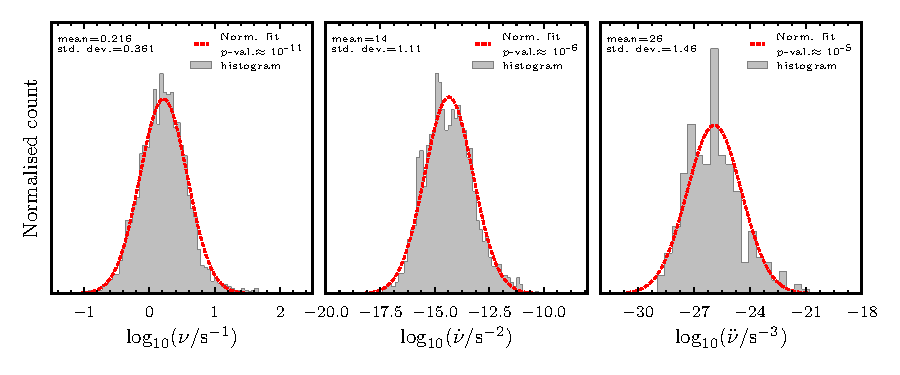
\includegraphics[]{timing_distribution}
\caption{The distribution in log-space of the frequency $\nu$ and the first two
frequency derivatives $\dot{\nu}$ and $\ddot{\nu}$ for normal radio pulsars in the
ATNF pulsar catalogue. Appropriate bin sizes were selected for each quantity.
The population sizes are 1942, 1686, 339 for $\nu$,
$\dot{\nu}$, $\ddot{\nu}$ respectively.}
\label{fig: pop stats timing}
\end{figure}
By eye, the histograms are clustered and appear to be approximately normal.
However, for all three properties, the normal hypothesis is rejected; we note
that the level of rejection is dependent on the number of data points. This
rejection is not surprising given the complicated physics which governs these
systems. The detailed population synthesis studies by \citet{faucher2006birth}
and \citet{popov2010population} are able to relate the observed features to the
underlying physics and find similar results for the period and period
derivative.

In Figure~\ref{fig: pop stats others} we present some other interesting quantities
held in the ATNF catalogue. Firstly, in the left-hand panel we plot the characteristic
age as defined in Eqn.~\eqref{eqn: tauAge definition}. Then, in the middle panel
we give a measure of the pulsar beam-width $W_{10}$. Specifically, $W_{10}$ is
the width of the integrated pulse profile (in seconds) at 10\% of the integrated
pulse profile maximum. In the right-hand panel we  plot $W_{10}\nu$, i.e. the
product of the beam-width and frequency for each pulsar. This gives information
about the effective duty-cycle: the ratio between the pulse duration and period.
Notably, the majority of pulsars have duty-cycles substantially less than a
$0.5$ indicating that the pulses are short compared to the period.
\begin{figure}[htb]
\centering
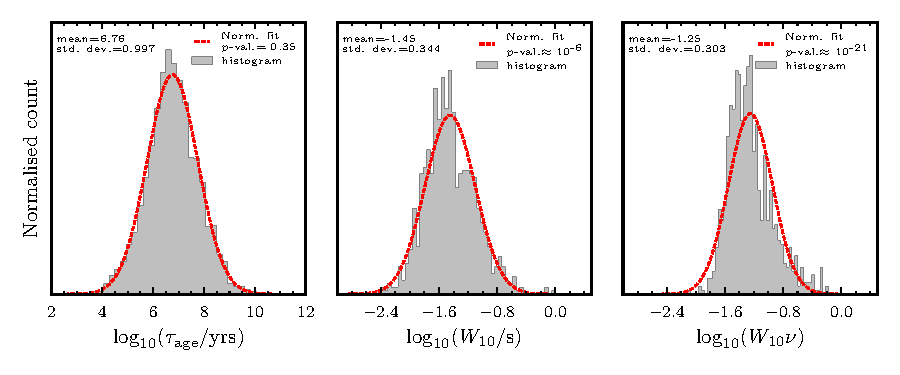
\includegraphics[]{W10_and_age_distribution}
\caption{The distribution in log-space of the characteristic age
$\tau_{\textrm{Age}}$, the $W_{10}$ measure of the beam-width, and the
effective duty-cycle $W_{10} \nu$ for normal radio pulsars in the
ATNF pulsar catalogue. Appropriate bin sizes were selected for each quantity.
The population sizes are 1942, 915, and 915 for
$\tau_{\textrm{Age}}$, $W_{10}$, and $W_{10}\nu$.}
\label{fig: pop stats others}
\end{figure}
In this instance, the normal hypothesis is rejected for the beam-width and
duty-cycle, but accepted for the spin-down age. It would be an interesting
exercise to investigate this further.

These results discussed in this section provide an overview of the observed
radio pulsar population. It must be remembered that these observed pulsars
are a sample from what may be a much larger population. These summaries are
intended only to give a brief overview of the observations.

